%! Author = paulsen
%! Date = 10.09.23

\begin{frame}{Einführung}
    \section{Einführung}\label{sec:einfuhrung}
\end{frame}

\begin{frame}{Vorstellung}
    \subsection{Vorstellung}\label{subsec:vorstellung}

    \underline{\textbf{Paul Seidel}}

    \begin{itemize}
        \item Internet Computing
        \item Linux seit 3 Jahren in der Uni \& Privat
        \item Ja, ich benutze auch Windows :)
    \end{itemize}

    \pause
    \vspace{0.5cm}
    \begin{alertblock}{Diskussion}
        Was ist euer Hintergrund?
    \end{alertblock}

\end{frame}

\begin{frame}{Erwartungen}
    \subsection{Erwartungen}\label{subsec:erwartungen}

    \begin{itemize}
        \item \begin{quote}
                  Linux ist was für Nerds!
        \end{quote}\pause
        \item \begin{quote}
                  Da macht man alles in der "Hacker"-Konsole!
        \end{quote}\pause
        \item \begin{quote}
                  Das ist mir zu viel Neuland!
        \end{quote}
    \end{itemize}

    \pause
    \vspace{0.5cm}
    \begin{alertblock}{Diskussion}
        Wie sieht es bei euch aus?
    \end{alertblock}

\end{frame}

\begin{frame}{Ziele}
    \subsection{Ziele}\label{subsec:ziele}

    \begin{enumerate}
        \item Schnelle Installation\pause
        \item Nutzung von Software\pause
        \item Umgang mit der Konsole\pause
        \item Systemkonfiguration\pause
        \item Beheben von Problemen\pause
        \item Gute Kenntnisse zum eigenständigen Arbeiten\pause
    \end{enumerate}

\end{frame}

\begin{frame}{Was ist Linux?}
    \subsection{Linux?}\label{subsec:linux?}

    \begin{quote}<1->
        Als GNU/Linux bezeichnet man in der Regel freie, unixähnliche Mehrbenutzer-Betriebssysteme, die auf dem Linux-Kernel und wesentlich auf GNU-Software basieren.
    \end{quote}

    \begin{itemize}
        \item<2-> 1991 als Alternative zu UNIX erschaffen
        \item<3-> Freie und offene Alternative zu Windows und MacOS
        \item<4-> Unterstützung von großen Unternehmen (Google, Microsoft, Facebook, etc.)
    \end{itemize}
    \begin{exampleblock}<1->{Fun Fact}
        Linux ist das größte Softwareprojekt der Welt.
    \end{exampleblock}

\end{frame}

\begin{frame}{Warum Linux?}
    \subsection{Warum Linux?}\label{subsec:warum-linux?}

    \begin{itemize}
        \item Performance und Stabilität
        \item Mehr Sicherheit und Flexibilität durch OpenSource
        \item Datenschutz (Keine Telemetriedaten)
    \end{itemize}

    \begin{exampleblock}<1->{Fun Fact}
        Linux im Weltall: ISS (Seit 1988) \& SpaceX (seit 2020).
    \end{exampleblock}

\end{frame}

\begin{frame}{Warum kein Linux?}
    \subsection{Warum kein Linux?}\label{subsec:warum-kein-linux?}

    \begin{itemize}
        \item Kein kompletter Microsoft-Office-Ersatz
        \item Wenn man es einfach haben will (In Linux kann man sehr Tüfteln)
        \item Mögliche Probleme beim Spielen
    \end{itemize}

\end{frame}

\begin{frame}{Linux Distributionen}
    \subsection{Distributionen}\label{subsec:distributionen}

    Ein großteil der Distributionen (Sorten) von Linux ist Teil dieser 3 "Familien":

    \pause

    \begin{itemize}
        \item Arch
        \item Debian
        \item RHEL (Red Hat Enterprise Linux)
    \end{itemize}

    \begin{exampleblock}<1->{Fun Fact}
        96,3\% des Internets läuft auf Linux-Servern
    \end{exampleblock}

\end{frame}


\begin{frame}{Desktop Umgebungen}
    \subsection{Desktop Umgebungen}\label{subsec:desktop-umgebungen}

    \begin{quote}
        Eine Desktop-Umgebung ist eine grafische Arbeits- bzw. Benutzerumgebung von Betriebssystemen in Form einer grafischen Shell [...]
    \end{quote}

    \begin{itemize}
        \item Desktops sind auch nur eigenständige Software in einer Linux-Distribution
        \item Leicht installierbar
    \end{itemize}

\end{frame}

\begin{frame}{Beispiele}
    \subsubsection{Beispiele}\label{subsubsec:beispiele}

    \href{https://opensource.com/article/20/5/linux-desktops}{Umfrage 2020 (opensource.com)}

    \begin{itemize}
        \item KDE Plasma (32\%)
        \item Gnome (24\%)
        \item KFCE (12\%)
        \item Cinnamon (11\%)
        \item sonst (21\%)
    \end{itemize}

\end{frame}

\begin{frame}{KDE Plasma}
    \subsubsection{KDE Plasma}\label{subsubsec:KDE-Plasma}

    \begin{tikzpicture}
        [remember picture, overlay, shift={(current page.north east)}]
        \node[anchor=north east,xshift=-.3cm,yshift=-2cm]{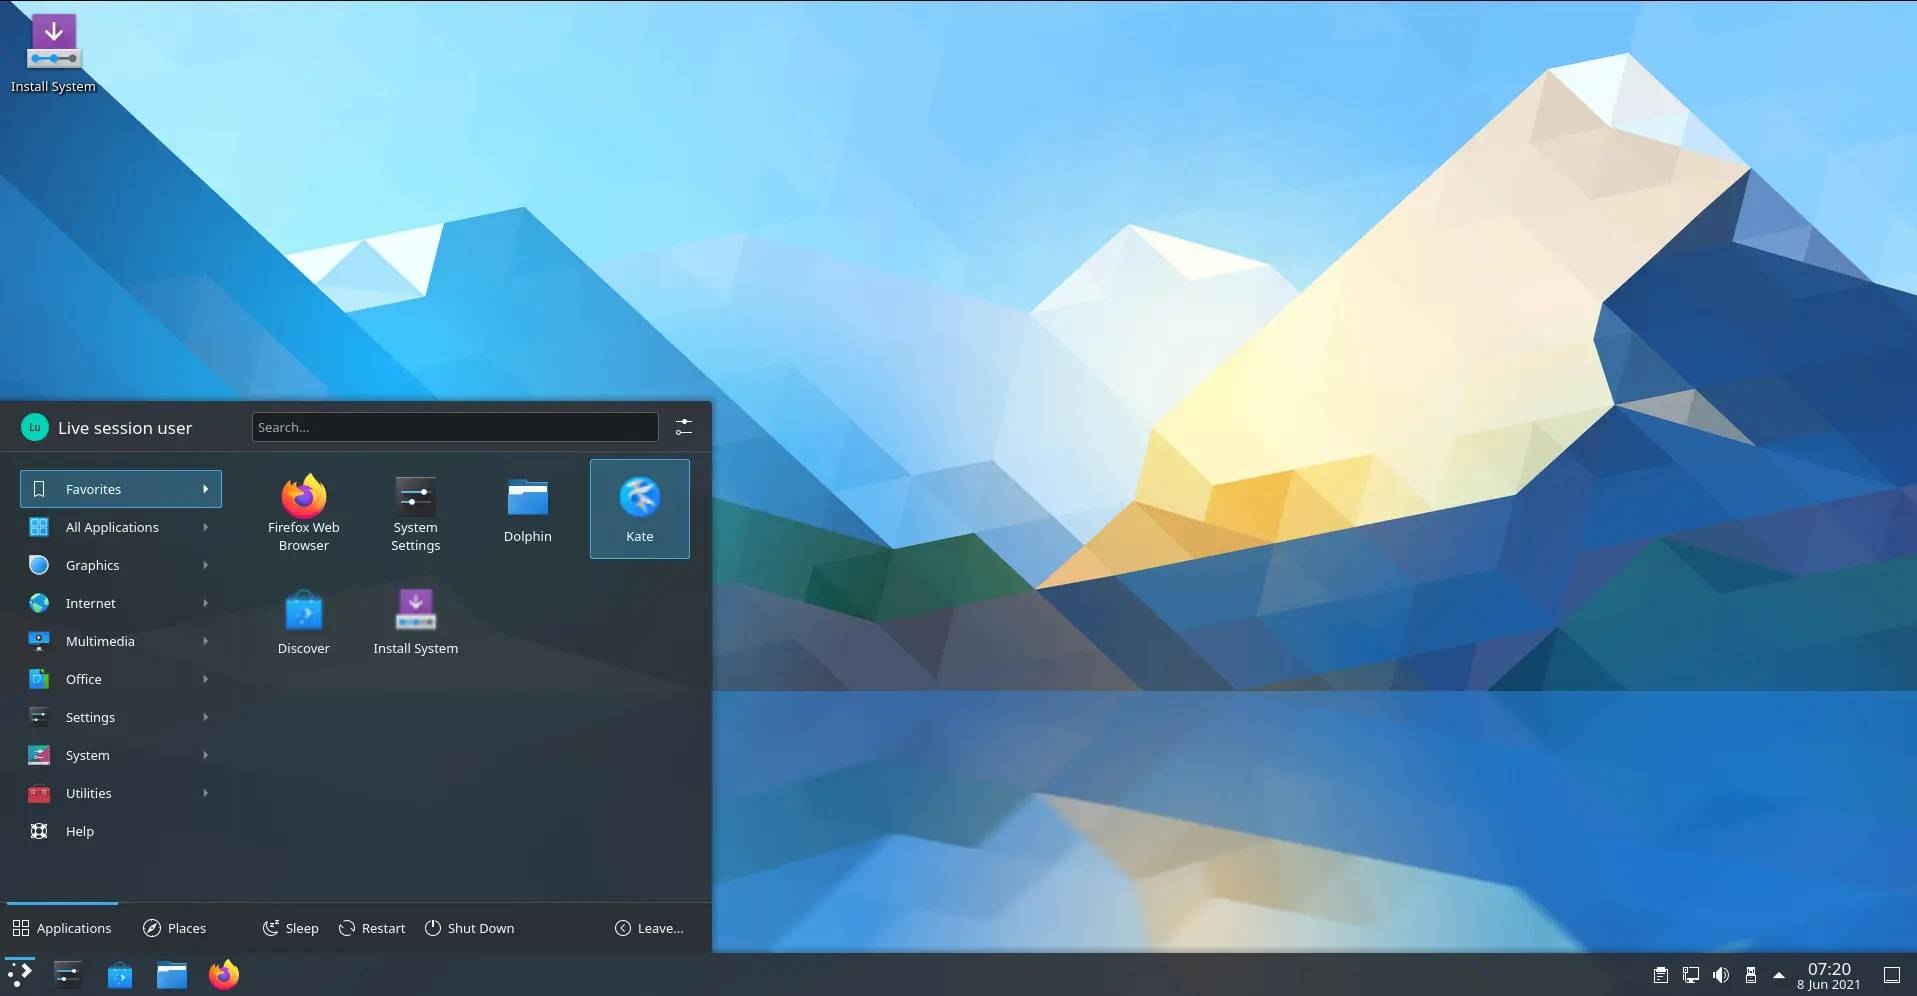
\includegraphics[width=12cm]{KDE-Plasma-Desktop}};
    \end{tikzpicture}

\end{frame}

\begin{frame}{Gnome}
    \subsubsection{Gnome}\label{subsubsec:Gnome}

    \begin{tikzpicture}
        [remember picture, overlay, shift={(current page.north east)}]
        \node[anchor=north east,xshift=-0.3cm,yshift=-2cm]{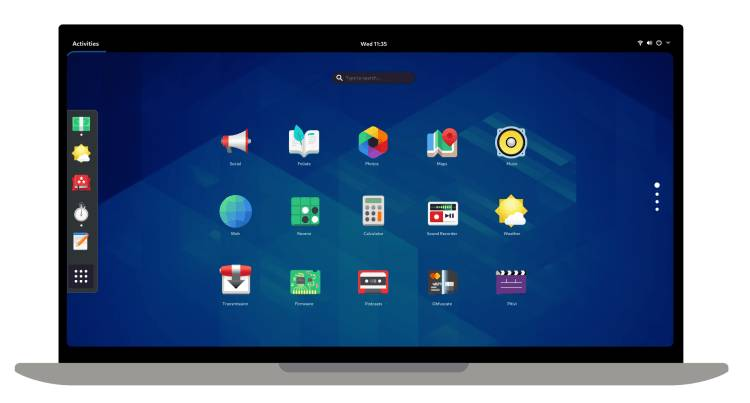
\includegraphics[width=12cm]{Gnome-Desktop}};
    \end{tikzpicture}

\end{frame}

\begin{frame}{XFCE}
    \subsubsection{XFCE}\label{subsubsec:XFCE}

    \begin{tikzpicture}
        [remember picture, overlay, shift={(current page.north east)}]
        \node[anchor=north east,xshift=-0.3cm,yshift=-1.7cm]{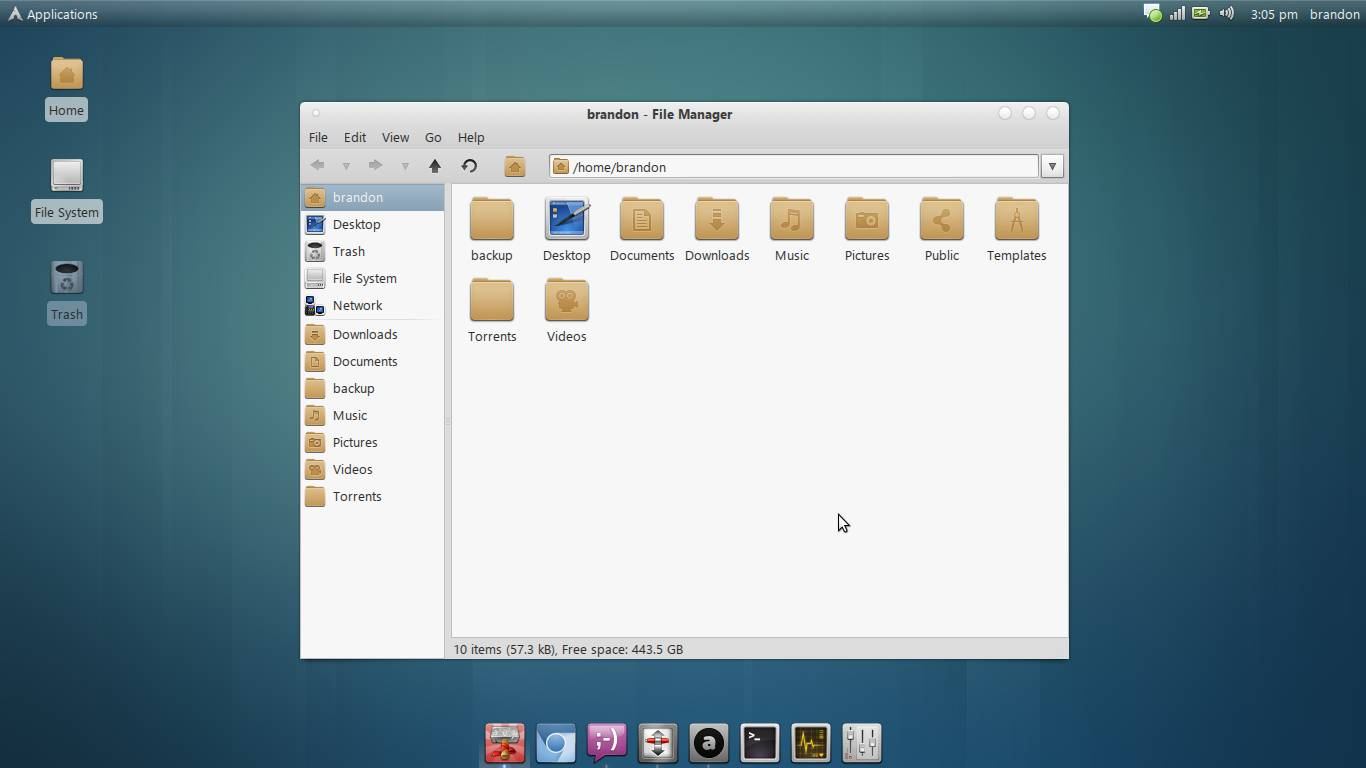
\includegraphics[width=12cm]{XFCE-Desktop}};
    \end{tikzpicture}

\end{frame}

\begin{frame}{Cinnamon}
    \subsubsection{Cinnamon}\label{subsubsec:Cinnamon}

    \begin{tikzpicture}
        [remember picture, overlay, shift={(current page.north east)}]
        \node[anchor=north east,xshift=-0.3cm,yshift=-1.7cm]{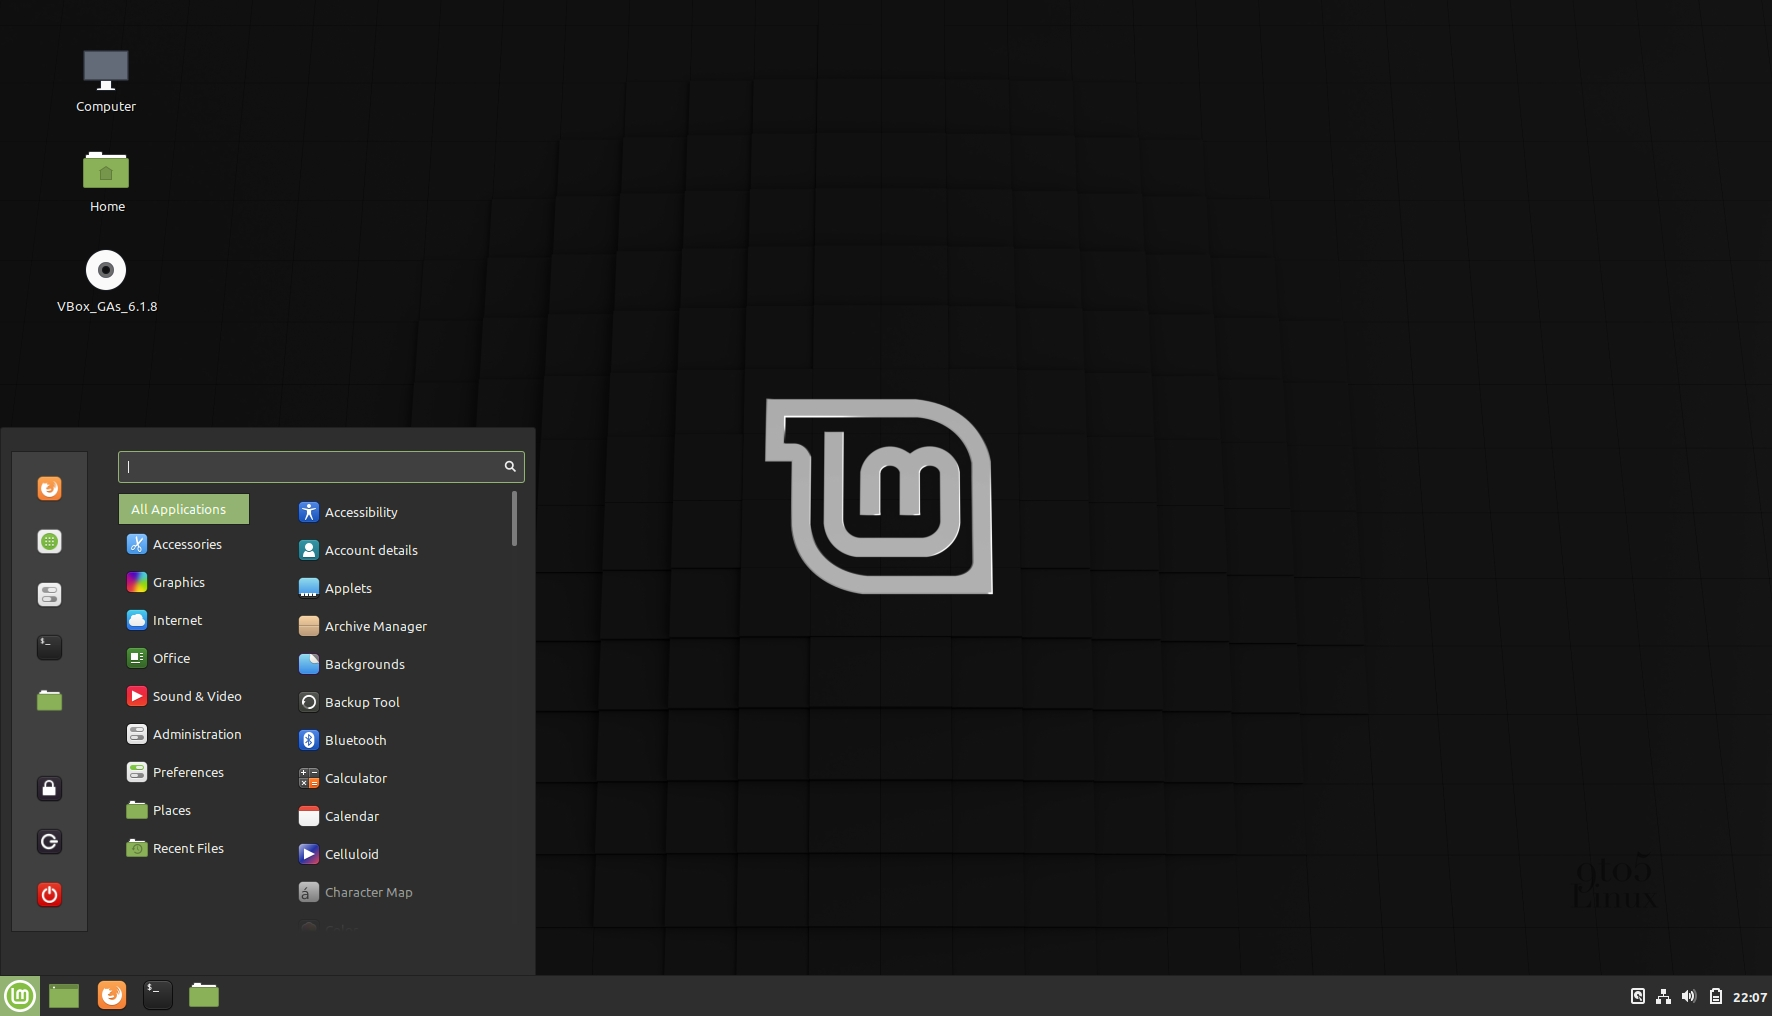
\includegraphics[width=12cm]{Mint-Desktop}};
    \end{tikzpicture}

\end{frame}


\begin{frame}{Other Desktops}
    \subsubsection{Other}\label{subsubsec:other}

    \begin{tikzpicture}
        [remember picture, overlay, shift={(current page.north east)}]
        \node[anchor=north east,xshift=-0.3cm,yshift=-1.7cm]{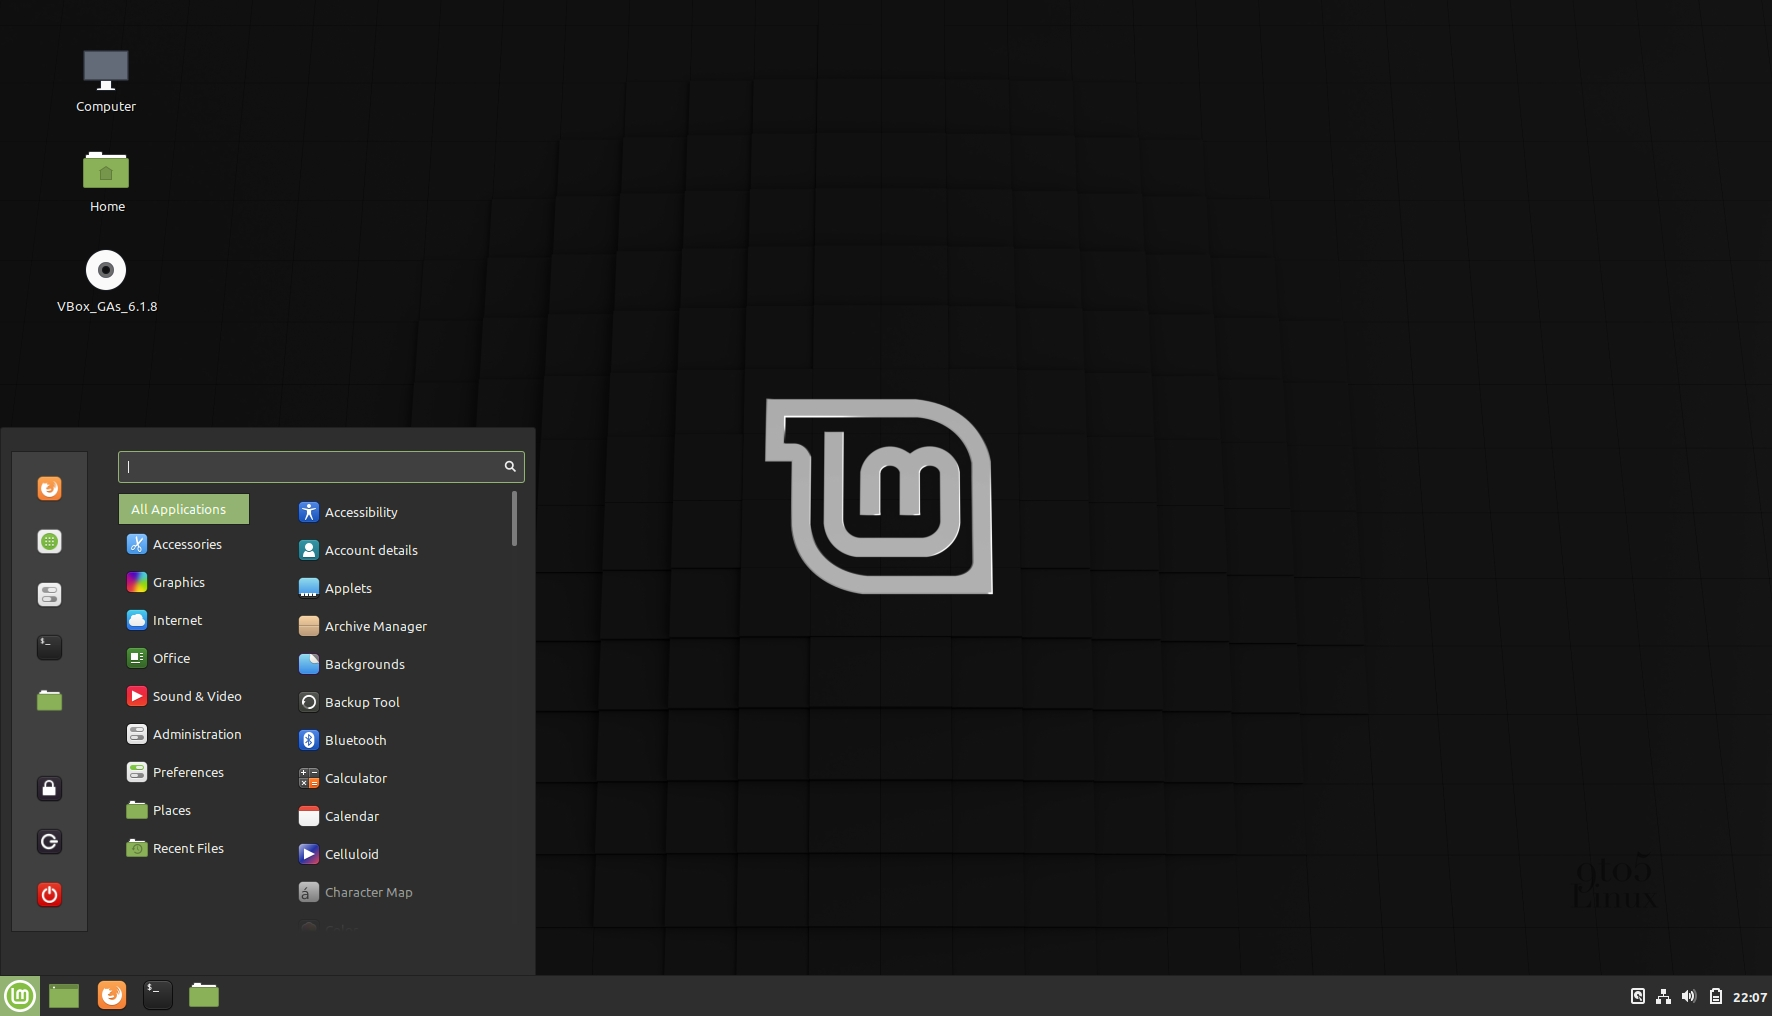
\includegraphics[width=12cm]{Mint-Desktop}};
    \end{tikzpicture}

\end{frame}